\documentclass[11pt]{beamer}
% \documentclass[11pt,handout]{beamer}
\usepackage[T1]{fontenc}
\usepackage[utf8]{inputenc}
\usepackage{float, afterpage, rotating, graphicx}
\usepackage{epstopdf}
\usepackage{longtable, booktabs, tabularx}
\usepackage{fancyvrb, moreverb, relsize}
\usepackage{eurosym, calc}
\usepackage{amsmath, amssymb, amsfonts, amsthm, bm}


\usepackage{natbib}
\bibliographystyle{rusnat}


\hypersetup{colorlinks=true, linkcolor=black, anchorcolor=black, citecolor=black, filecolor=black, menucolor=black, runcolor=black, urlcolor=black}

\setbeamertemplate{footline}[frame number]
\setbeamertemplate{navigation symbols}{}
\setbeamertemplate{frametitle}{\centering\vspace{1ex}\insertframetitle\par}


\begin{document}

\title{The Effectiveness of Strategies to Contain SARS-CoV-2: Testing, Vaccinations, and NPIs}

\author[Janoś Gabler, Tobias Raabe, Klara Röhrl, Hans-Martin von Gaudecker]
{
{\bf Janoś Gabler, Tobias Raabe, Klara Röhrl, Hans-Martin von Gaudecker}\\
{\small Universität Bonn and IZA}\\[1ex]
}


\begin{frame}
    \titlepage
    \note{~}
\end{frame}


\begin{frame}{Agentenbasiertes Modell}
    \vskip.1cm
    \centering
    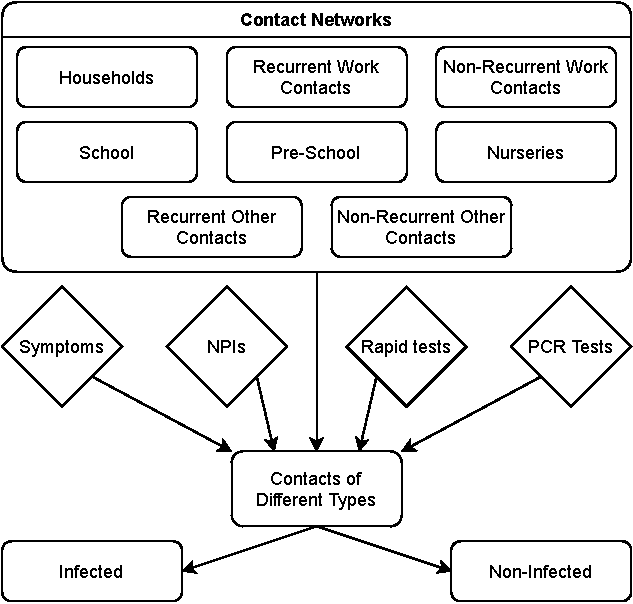
\includegraphics[height=.9\textheight]{figures/model-graph-top-left}
\end{frame}


\begin{frame}{Krankheitsverlauf}
    \centering
    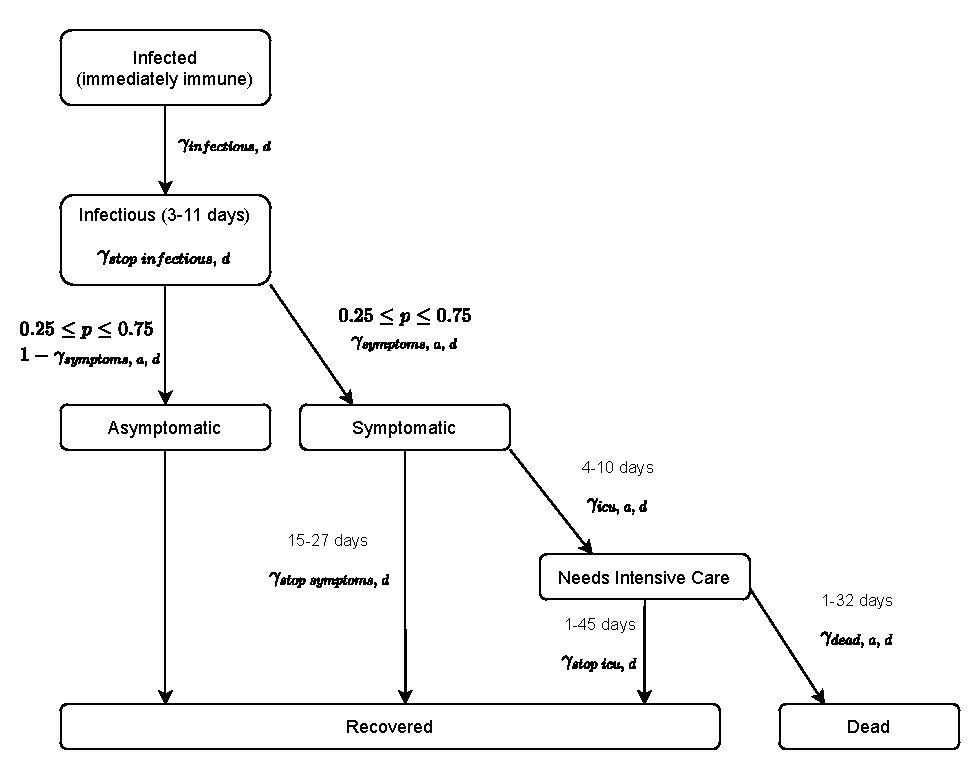
\includegraphics[width=\textwidth]{figures/model-graph-top-right}
\end{frame}


\begin{frame}{Testnachfrage}
    \centering
    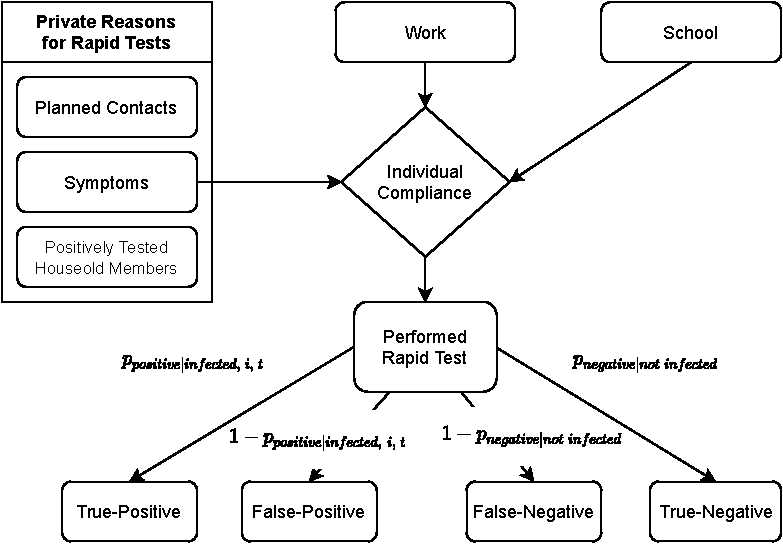
\includegraphics[width=\textwidth]{figures/model-graph-bottom-left}
\end{frame}


\begin{frame}{Offizielle Fälle $\rightarrow$ Gesamtzahl}
    \centering
    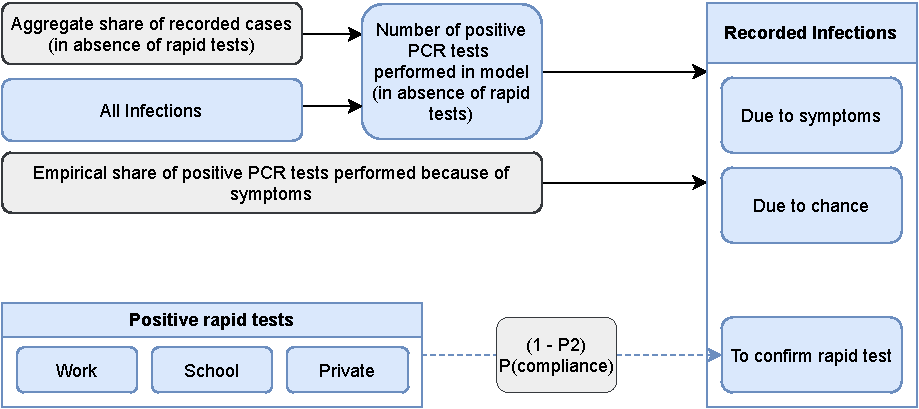
\includegraphics[width=\textwidth]{figures/model-graph-bottom-right}
\end{frame}


\begin{frame}{Fallzahlen: Modell vs. Daten}
    \centering
    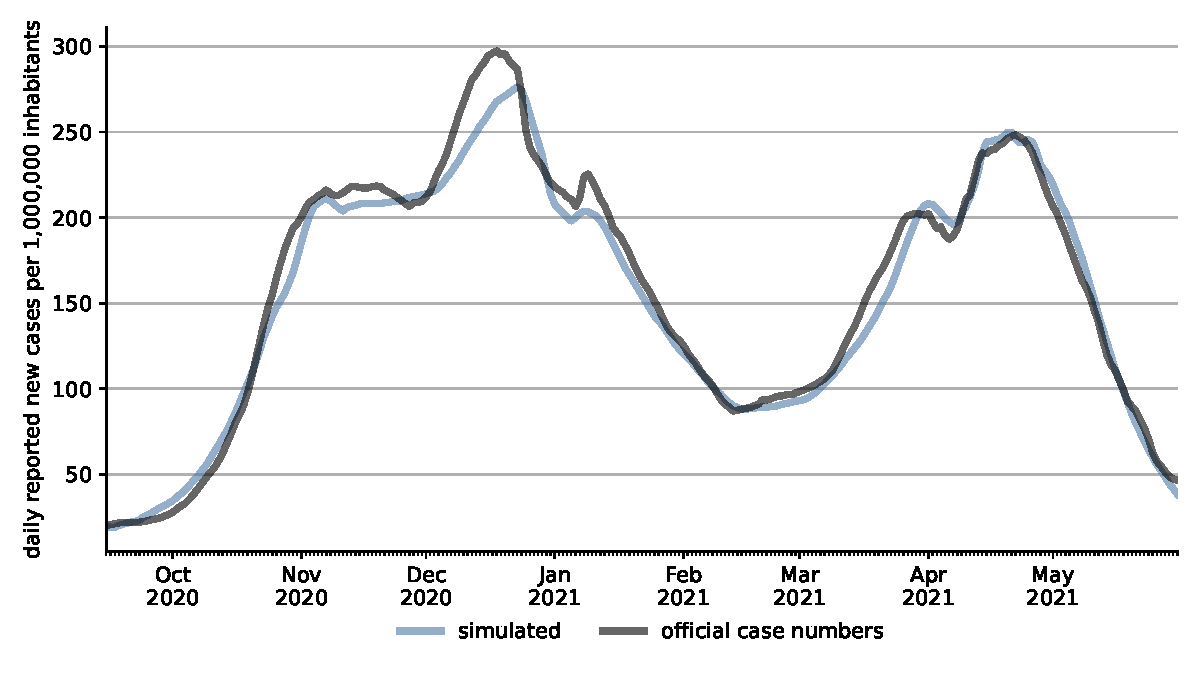
\includegraphics[width=\textwidth]{figures/results/figures/scenario_comparisons/combined_fit/full_new_known_case}
\end{frame}


\begin{frame}{Verlauf Lockdownmaßnahmen}
    \centering
    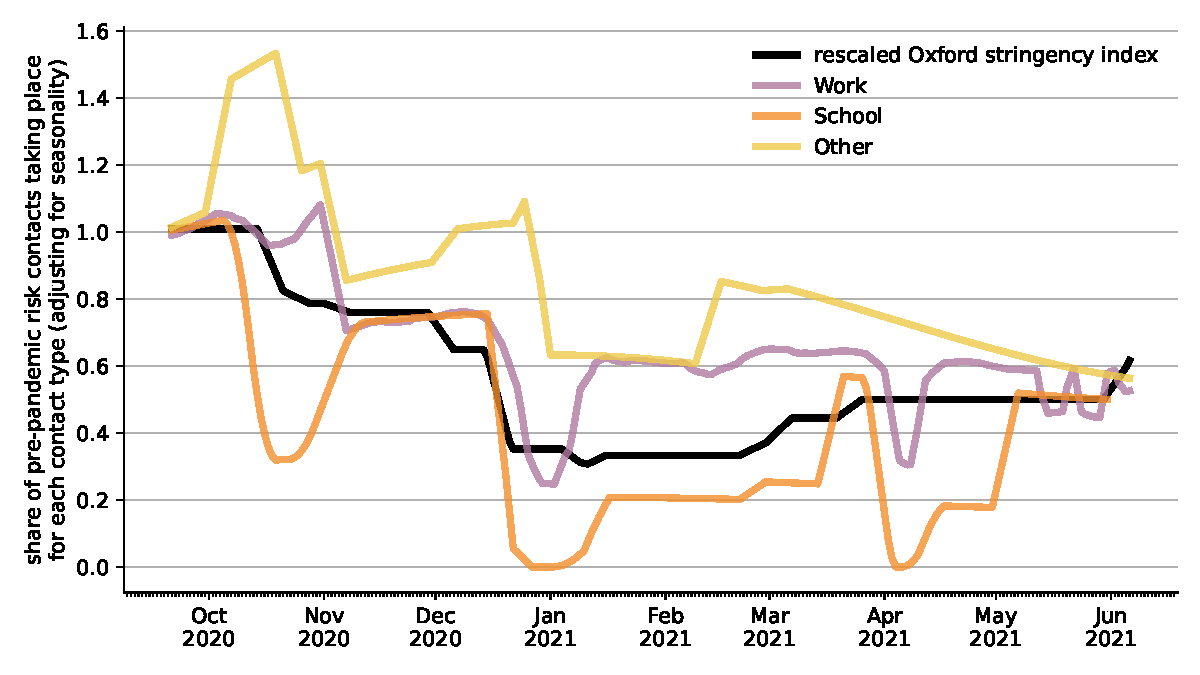
\includegraphics[width=\textwidth]{figures/results/figures/data/stringency2_with_seasonality}
\end{frame}


\begin{frame}{Anteil Alpha: Modell vs. Daten}
    \centering
    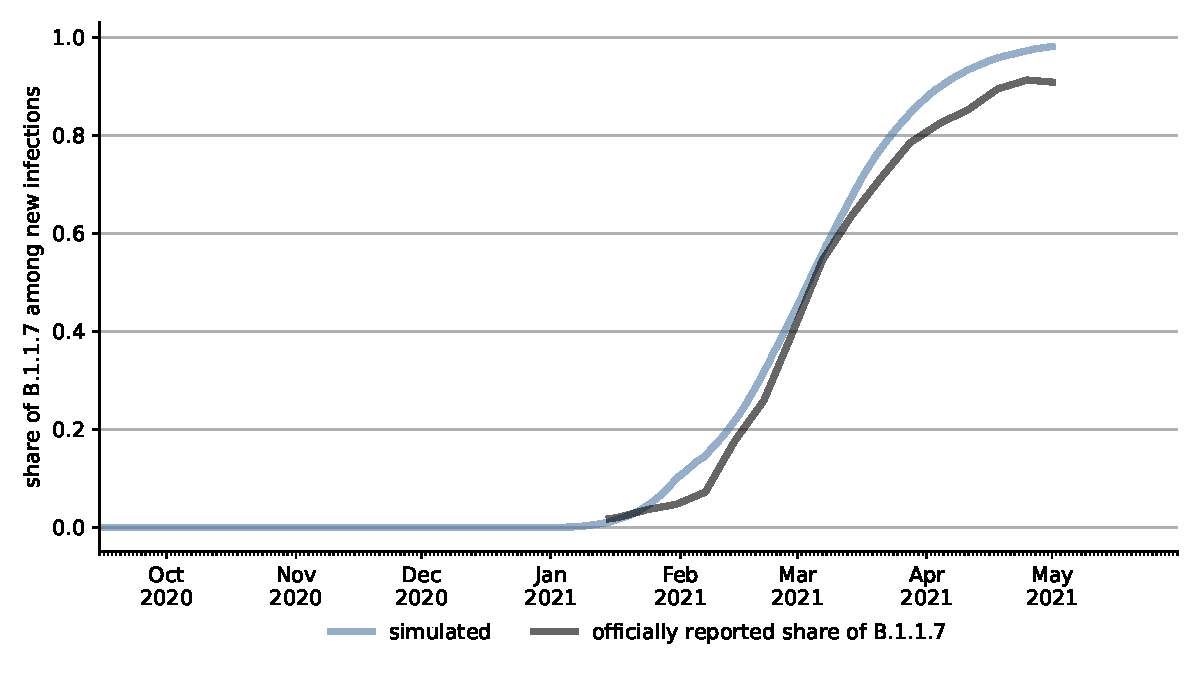
\includegraphics[width=\textwidth]{figures/results/figures/scenario_comparisons/combined_fit/full_share_b117}
\end{frame}


\begin{frame}{Testen, Impfen: Modell vs. Daten}
    \centering
    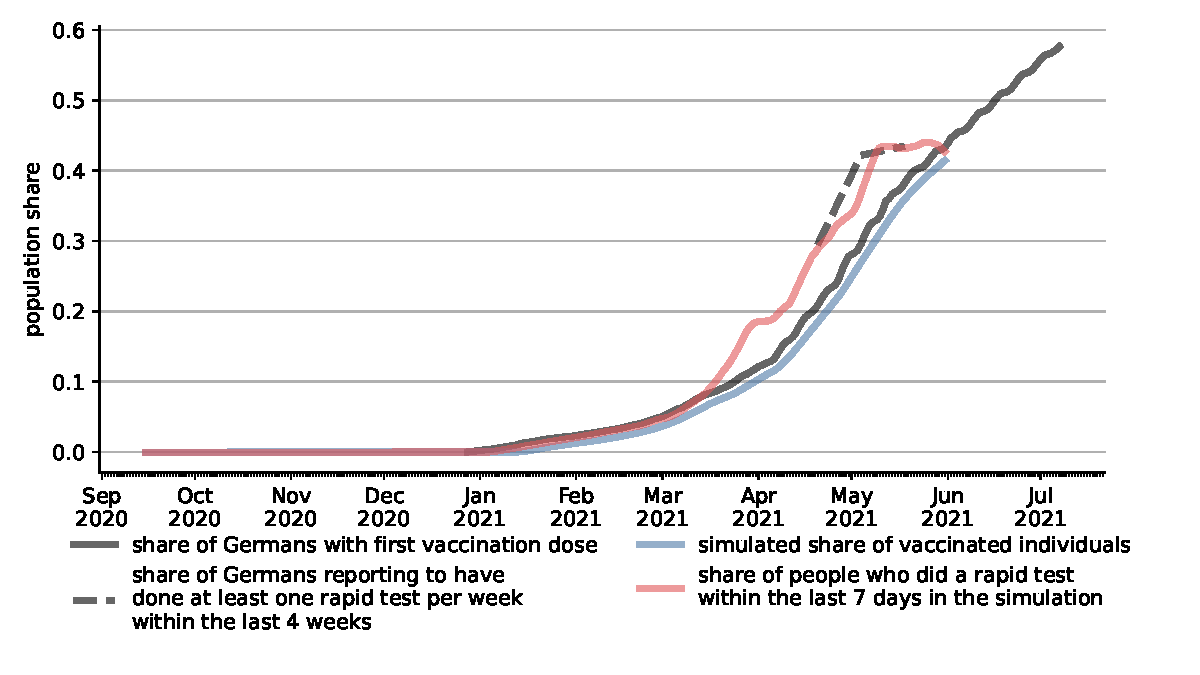
\includegraphics[width=\textwidth]{figures/results/figures/scenario_comparisons/combined_fit/full_share_rapid_test_in_last_week_and_vaccinated}
\end{frame}


\begin{frame}{Szenarien Frühjahr 2021: Offizielle Fälle}
    \centering
    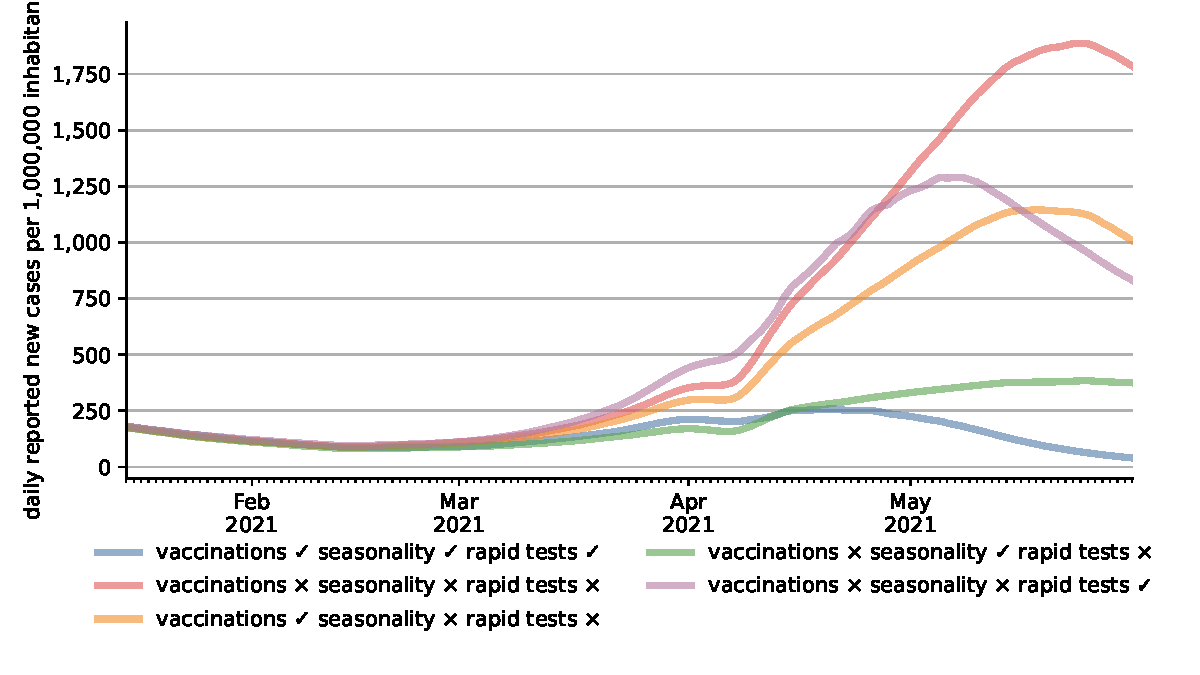
\includegraphics[width=\textwidth]{figures/results/figures/scenario_comparisons/effect_of_channels_on_pessimistic_scenario/full_new_known_case}
\end{frame}


\begin{frame}{Szenarien Frühjahr 2021: Alle Fälle}
    \centering
    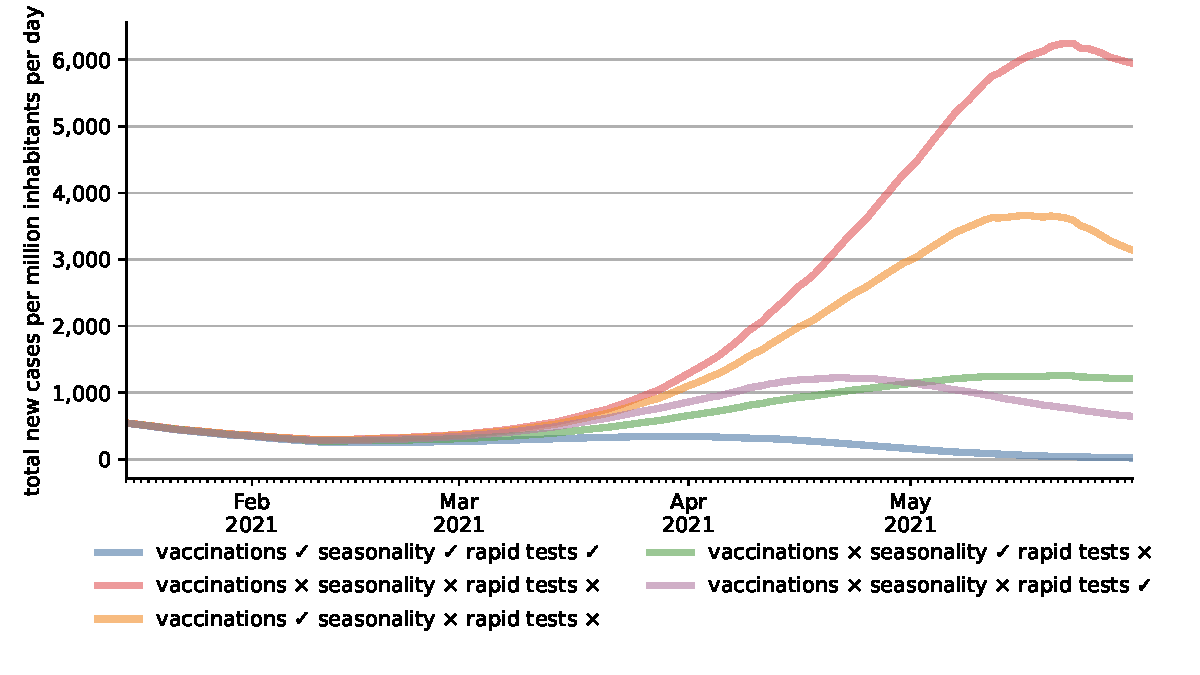
\includegraphics[width=\textwidth]{figures/results/figures/scenario_comparisons/effect_of_channels_on_pessimistic_scenario/full_newly_infected}
\end{frame}


\begin{frame}{Szenarien Frühjahr 2021: Zerlegung Einflussfaktoren}
    \centering
    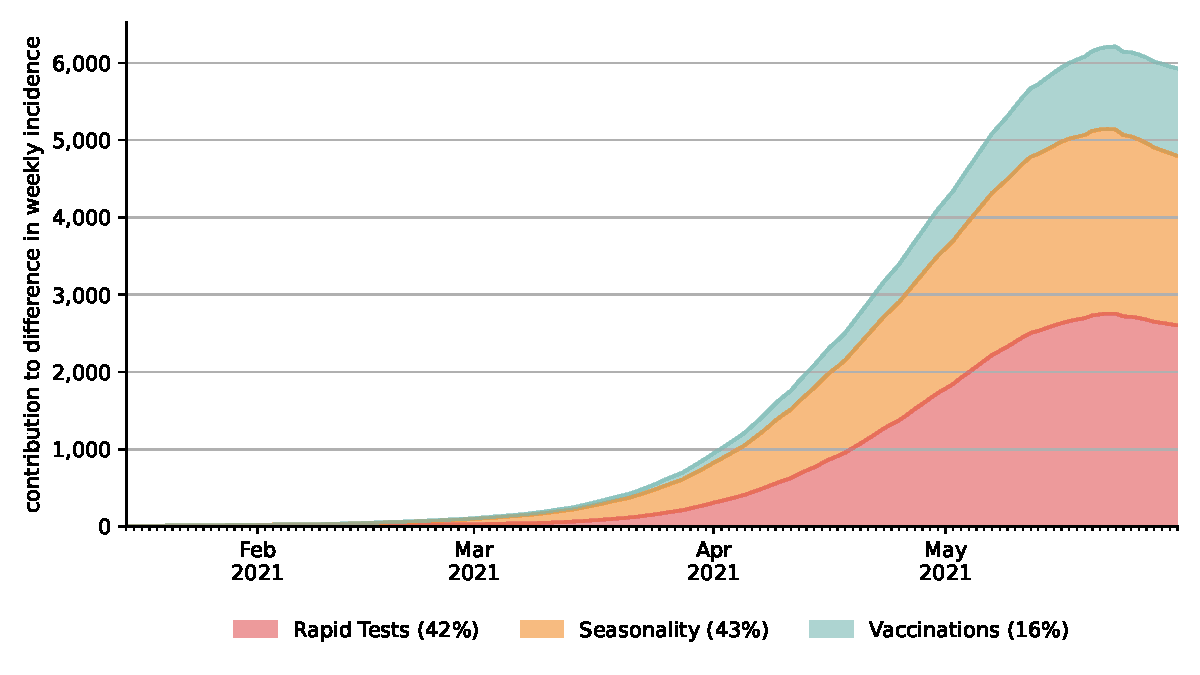
\includegraphics[width=\textwidth]{figures/results/figures/full_decomposition_channels_area}
\end{frame}


\begin{frame}{Szenarien Frühjahr 2021: Zerlegung Tests}
    \centering
    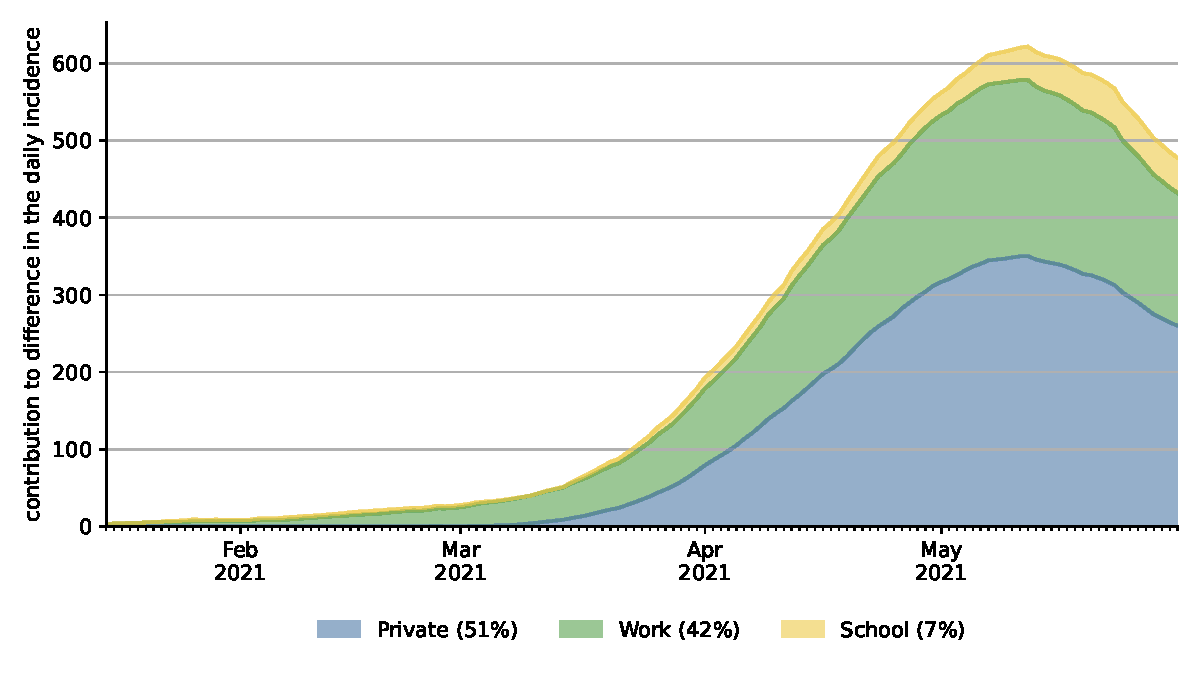
\includegraphics[width=\textwidth]{figures/results/figures/full_decomposition_rapid_tests_area}
\end{frame}


\begin{frame}\frametitle{Nächste Schritte}
    \begin{itemize}
        \item Einbau Delta (Infektiösität, Latenzzeit) \\[3ex]
        \item Bessere Parameter geimpft / genesen \\[3ex]
        \item Automatismen in Regeln (NPIs basierend auf Intensivbelegung)
    \end{itemize}
\end{frame}

% Print black screen only in presentation mode for finishing up.
\mode<beamer> {
    \beamersetaveragebackground{black}
    \begin{frame}
        \frametitle{}
    \end{frame}

    \beamersetaveragebackground{white}
}

% \begin{frame}[allowframebreaks]
%     \frametitle{References}


%     \bibliography{refs}
% \end{frame}

\end{document}
